\documentclass[11pt,addpoints]{exam}
\usepackage{fullpage}
\usepackage{amsfonts, amsmath, amssymb, amsthm}
\usepackage{mathtools}
\usepackage{enumerate}
\usepackage{listings}
\usepackage[boxed]{algorithm}
\usepackage[noend]{algpseudocode}
\usepackage[inline]{enumitem}
\usepackage{hyperref}
\usepackage{tikz}
\usetikzlibrary{decorations.pathreplacing, positioning}
\newcommand*\circled[1]{\tikz[baseline=(char.base)]{
            \node[shape=circle,draw,inner sep=2pt] (char) {#1};}}

% in order to compile this file you need to get 'header.tex' from
% Canvas and change the line below to the appropriate file path
%%% theorems

\theoremstyle{plain}            % following are "theorem" style
\newtheorem{theorem}{Theorem}[section]
\newtheorem{lemma}[theorem]{Lemma}
\newtheorem{corollary}[theorem]{Corollary}
\newtheorem{proposition}[theorem]{Proposition}
\newtheorem{claim}[theorem]{Claim}
\newtheorem{fact}[theorem]{Fact}
\newtheorem{openproblem}[theorem]{Open Problem}

\theoremstyle{definition}       % following are def style
\newtheorem{definition}[theorem]{Definition}
\newtheorem{conjecture}[theorem]{Conjecture}
\newtheorem{example}[theorem]{Example}
\newtheorem{protocol}[theorem]{Protocol}
\newtheorem{exercise}[theorem]{Exercise}

\theoremstyle{remark}           % following are remark style
\newtheorem{remark}[theorem]{Remark}
\newtheorem{note}[theorem]{Note}
\newtheorem*{aside}{Aside}
\newtheorem*{gn}{Grading Note} % grading note

%%% special sets
\newcommand{\bit}{\ensuremath{\{0,1\}}}
\newcommand{\bitt}{\ensuremath{\{-1,1\}}}

% font for general-purpose algorithms
\newcommand{\algo}[1]{\ensuremath{\mathsf{#1}}}
% font for general-purpose computational problems
\newcommand{\problem}[1]{\ensuremath{\mathsf{#1}}}
% font for complexity classes
%\newcommand{\class}[1]{\ensuremath{\mathsf{#1}}}

\global\long\def\path{\mathrm{path}}
% asymptotics
%\DeclareMathOperator{\poly}{poly}
%\DeclareMathOperator{\polylog}{polylog}
\DeclareMathOperator{\negl}{negl}
\DeclareMathOperator{\Otil}{\tilde{O}}
\DeclareMathOperator{\Ostar}{O^*}

%%% "LEFT-RIGHT" PAIRS OF SYMBOLS

% inner product
\DeclarePairedDelimiter\inner{\langle}{\rangle}
% absolute value
\DeclarePairedDelimiter\abs{\lvert}{\rvert}
% a set
\DeclarePairedDelimiter\set{\{}{\}}
% parens
\DeclarePairedDelimiter\parens{(}{)}
% tuple, alias for parens
\DeclarePairedDelimiter\tuple{(}{)}
% square brackets
\DeclarePairedDelimiter\bracks{[}{]}
% rounding off
\DeclarePairedDelimiter\round{\lfloor}{\rceil}
% floor function
\DeclarePairedDelimiter\floor{\lfloor}{\rfloor}
% ceiling function
\DeclarePairedDelimiter\ceil{\lceil}{\rceil}
% length of some vector, element
\DeclarePairedDelimiter\length{\lVert}{\rVert}
% norm
\DeclarePairedDelimiter\norm{\lVert}{\rVert}
% length (as a string)
\DeclarePairedDelimiter\len{\lvert}{\rvert}
% bra-kets
\DeclarePairedDelimiter\bra{\langle}{\rvert}
\DeclarePairedDelimiter\ket{\lvert}{\rangle}
\newcommand{\braket}[2]{\ensuremath{\langle #1 \vert #2 \rangle}}
\newcommand{\ketbra}[2]{\ensuremath{\lvert #1 \rangle \langle #2 \rvert}}

%%% MATH OPERATORS
\DeclareMathOperator{\Var}{Var}
\DeclareMathOperator{\tr}{Tr}
\DeclareMathOperator{\supp}{supp}
\DeclareMathOperator{\var}{var}
\DeclareMathOperator{\vol}{vol}
\DeclareMathOperator{\sign}{sign}

%%% BLACKBOARD SYMBOLS

\newcommand{\C}{\ensuremath{\mathbb{C}}}
\newcommand{\D}{\ensuremath{\mathbb{D}}}
\newcommand{\F}{\ensuremath{\mathbb{F}}}
\newcommand{\G}{\ensuremath{\mathbb{G}}}
\newcommand{\J}{\ensuremath{\mathbb{J}}}
\newcommand{\N}{\ensuremath{\mathbb{N}}}
\newcommand{\Q}{\ensuremath{\mathbb{Q}}}
\newcommand{\R}{\ensuremath{\mathbb{R}}}
\newcommand{\T}{\ensuremath{\mathbb{T}}}
\newcommand{\Z}{\ensuremath{\mathbb{Z}}}
\newcommand{\QR}{\ensuremath{\mathbb{QR}}}

% sets in calligraphic type

\newcommand{\calD}{\ensuremath{\mathcal{D}}}
\newcommand{\calF}{\ensuremath{\mathcal{F}}}
\newcommand{\calG}{\ensuremath{\mathcal{G}}}
\newcommand{\calH}{\ensuremath{\mathcal{H}}}
\newcommand{\calI}{\ensuremath{\mathcal{I}}}
\newcommand{\calL}{\ensuremath{\mathcal{L}}}
\newcommand{\calN}{\ensuremath{\mathcal{N}}}
\newcommand{\calP}{\ensuremath{\mathcal{P}}}
\newcommand{\calS}{\ensuremath{\mathcal{S}}}
\newcommand{\calX}{\ensuremath{\mathcal{X}}}
\newcommand{\calY}{\ensuremath{\mathcal{Y}}}

% matrices and vectors

\newcommand{\matA}{\ensuremath{\mathbf{A}}}
\newcommand{\matB}{\ensuremath{\mathbf{B}}}
\newcommand{\matC}{\ensuremath{\mathbf{C}}}
\newcommand{\matD}{\ensuremath{\mathbf{D}}}
\newcommand{\matE}{\ensuremath{\mathbf{E}}}
\newcommand{\matF}{\ensuremath{\mathbf{F}}}
\newcommand{\matG}{\ensuremath{\mathbf{G}}}
\newcommand{\matH}{\ensuremath{\mathbf{H}}}
\newcommand{\matI}{\ensuremath{\mathbf{I}}}
\newcommand{\matJ}{\ensuremath{\mathbf{J}}}
\newcommand{\matK}{\ensuremath{\mathbf{K}}}
\newcommand{\matL}{\ensuremath{\mathbf{L}}}
\newcommand{\matM}{\ensuremath{\mathbf{M}}}
\newcommand{\matN}{\ensuremath{\mathbf{N}}}
\newcommand{\matO}{\ensuremath{\mathbf{O}}}
\newcommand{\matP}{\ensuremath{\mathbf{P}}}
\newcommand{\matQ}{\ensuremath{\mathbf{Q}}}
\newcommand{\matR}{\ensuremath{\mathbf{R}}}
\newcommand{\matS}{\ensuremath{\mathbf{S}}}
\newcommand{\matT}{\ensuremath{\mathbf{T}}}
\newcommand{\matU}{\ensuremath{\mathbf{U}}}
\newcommand{\matV}{\ensuremath{\mathbf{V}}}
\newcommand{\matW}{\ensuremath{\mathbf{W}}}
\newcommand{\matX}{\ensuremath{\mathbf{X}}}
\newcommand{\matY}{\ensuremath{\mathbf{Y}}}
\newcommand{\matZ}{\ensuremath{\mathbf{Z}}}
\newcommand{\matzero}{\ensuremath{\mathbf{0}}}

\newcommand{\veca}{\ensuremath{\mathbf{a}}}
\newcommand{\vecb}{\ensuremath{\mathbf{b}}}
\newcommand{\vecc}{\ensuremath{\mathbf{c}}}
\newcommand{\vecd}{\ensuremath{\mathbf{d}}}
\newcommand{\vece}{\ensuremath{\mathbf{e}}}
\newcommand{\vecf}{\ensuremath{\mathbf{f}}}
\newcommand{\vecg}{\ensuremath{\mathbf{g}}}
\newcommand{\vech}{\ensuremath{\mathbf{h}}}
\newcommand{\veck}{\ensuremath{\mathbf{k}}}
\newcommand{\vecm}{\ensuremath{\mathbf{m}}}
\newcommand{\vecp}{\ensuremath{\mathbf{p}}}
\newcommand{\vecq}{\ensuremath{\mathbf{q}}}
\newcommand{\vecr}{\ensuremath{\mathbf{r}}}
\newcommand{\vecs}{\ensuremath{\mathbf{s}}}
\newcommand{\vect}{\ensuremath{\mathbf{t}}}
\newcommand{\vecu}{\ensuremath{\mathbf{u}}}
\newcommand{\vecv}{\ensuremath{\mathbf{v}}}
\newcommand{\vecw}{\ensuremath{\mathbf{w}}}
\newcommand{\vecx}{\ensuremath{\mathbf{x}}}
\newcommand{\vecy}{\ensuremath{\mathbf{y}}}
\newcommand{\vecz}{\ensuremath{\mathbf{z}}}
\newcommand{\veczero}{\ensuremath{\mathbf{0}}}
\newcommand{\vecone}{\ensuremath{\mathbf{1}}}

%%% misc

\newcommand{\eps}{\varepsilon}

%%% for homework and section notes

\newcommand{\commonheader}[2]{
    \pagestyle{headandfoot}
    \setlength{\headheight}{26pt}
    \setlength{\headsep}{16pt}

    \header
        {\small{\textbf{EECS 376: Foundations of Computer Science}} \\ \footnotesize{\textbf{University of Michigan, Spring 2024}}}
        {#1}
        {#2}

    \firstpageheadrule
    \runningheadrule

    \footer
        {}
        {\thepage}
        {}
}

\newcommand{\hwheader}{
    \commonheader
        {\Large \textbf{Homework \hwnum}}
        {\small \textbf{Due 8:00pm, \duedate\\ {\tiny(accepted until 9:59 pm, no credit after)}}}
}

\newcommand{\hwslnheader}{
    \commonheader
    	{}
        {\Large \textbf{Solutions to Homework \hwnum}}
    \printanswers
}

\newcommand{\notesheader}{
    \commonheader
    	{}
        {\Large \textbf{Discussion Notes \sectionnum}}
}

\newcommand{\practiceheader}{
    \commonheader
    	{}
        {\Large \textbf{Discussion Worksheet \sectionnum}}
}

\newcommand{\practiceslnheader}{
    \commonheader
    	{}
        {\Large \textbf{Solutions to Discussion Worksheet \sectionnum}}
}

\newcommand{\reviewheader}{
    \commonheader 
    \smallskip
    	{}
        {\Large \textbf{Midterm Review Notes}}
}

\newcommand{\hwpreface}{

\noindent This homework has \numquestions\ questions, for a total of \numpoints\ points and \numbonuspoints\ extra-credit points.

\noindent Unless otherwise stated, each question requires \emph{clear}, \emph{logically correct}, and \emph{sufficient} justification to convince the reader.

\noindent For bonus/extra-credit questions, we will provide very limited guidance in office hours and on Piazza, and we do not guarantee anything about the difficulty of these questions.
 
\noindent We strongly encourage you to typeset your solutions in \LaTeX.

\noindent If you collaborated with someone, you must state their name(s). You must \emph{write your own solution} for all problems and \emph{may not use any other student’s write-up}.
}

\newcommand{\hint}[1]{
\emph{Hint}: #1
}
\newcommand{\bonus}{
\emph{Optional bonus}:
}
\newcommand{\extracredit}{
\emph{Extra credit}: 
}


\newcommand{\hwnum}{2}
\newcommand{\duedate}{May 23}
\usepackage{xcolor}

% remove "draft" to turn off fixme notes
\usepackage[draft,multiuser,inline,nomargin]{fixme}
% fixme notes: register commands for author(s)
% \FXRegisterAuthor{}{}{}
% add more HW authors here...
% TODO: this week's HW team- pick a color for yourself.
\fxusetheme{color}

\algrenewcommand\algorithmicrequire{\textbf{Input:}}
\algrenewcommand\algorithmicensure{\textbf{Output:}}

\hwheader   % header for homework
% \hwslnheader   % header for homework solutions

% Comment the following line in order to hide solutions.
% Uncomment the line to show solutions written inside of
% LaTeX solution environments like:
%   \begin{solution}
%     My solution.
%   \end{solution}.
\printanswers

\begin{document}

\listoffixmes

\hwpreface

\pointsinmargin
\pointpoints{pt}{pts}
\bonuspointpoints{EC pt}{EC pts}
\marginpointname{ \points}
\marginbonuspointname{ \bonuspoints}

\begin{questions}
  \addtocounter{question}{-1}
  \question[0] \textbf{Before you start; before you submit.}
  
  \begin{parts}
    \part Carefully review Sections 1.2-1.3 (Induction for Reasoning about Algorithms) of  \href{https://drive.google.com/file/d/1Q6E2B2hljH28vv7L1LZOugiJol-t1khq/view?usp=drive_link}{Handout~1} before starting this assignment, and apply it to the solutions you submit.
    
    \part If applicable, state the name(s) and uniqname(s) of your collaborator(s).

    \begin{solution}
      None.
    \end{solution}
  \end{parts}

  \question[10] \textbf{Self assessment.}

  Carefully read and understand the posted solutions to the previous homework.
  Identify one part for which your own solution has the most room for improvement (e.g., has unsound reasoning, doesn’t show what was required, could be significantly clearer or better organized, etc.).
  Copy or screenshot this solution, then in a few sentences, explain what was deficient and how it could be fixed.

  (Alternatively, if you think one of your solutions is significantly \emph{better} than the posted one, copy it here and explain why you think it is better.)

  \begin{solution}
      I checked the solution and gladly found that my solution was correct and well-organized for most parts, except in question 2 where I did not consider that \(T_Z(n) = O(n^2 \log n)\) which uses the big-O notation which is the asymptotical upper bound while the \(T_Y(n) = \Theta(n^2)\) uses the big-Theta notation which is the asymptotically tight bound. So this time I should be more careful in reading the questions and reasoning.
  \end{solution}
    
    \question \textbf{Binary Tree Configuration Count.}
    
    Let $T(n)$ be the number of (rooted) binary tree configurations with exactly $n$ nodes. Examples of the first few values of $T$ are shown below – two trees are distinct if a single node changes position, with right and left children considered distinguishable. 

\begin{center}
\includegraphics[scale=0.6]{MC-4.png}\\
$T(0) = 1, T(1) = 1, T(2) = 2, T(3) = 5$
\end{center}

 $T(n)$ can be described by the following recurrence:
 \[T(n) = T(0)T(n - 1) + T(1)T(n - 2) + ... + T(n - 1)T(0).\]
 \begin{parts}
     \part[5] Give a combinatorial argument for why this recurrence correctly counts the number of trees with $n$ nodes.
     \part[5] Write down pseudocode to compute $T(n)$, using dynamic programming. Your implementation should have runtime $O(n^2)$; briefly justify why this is true.
     \part[5] Now consider a variation on this problem: write down a recurrence to count the number of \emph{non-empty} binary trees where every node has 0 or 2 children. Briefly explain why your recurrence is correct.
 \end{parts}

\begin{solution}
  \begin{parts}
    \part 
    $$
    T(n) = \sum_{k=0}^{n-1} T(k)T(n-k-1)
    $$
    $T(n)$ is the number of binary trees with $n$ nodes. There must be a root node which is always in the same position. So we we can view $T(n)$ as the number of ways to arrange for the left and right subtrees of the root by $n-1$ nodes. 
    \\\\If we put $k$ nodes in the left subtree of the root, then there are $n-k-1$ nodes in the right subtree. So the number of ways to arrange the left subtree with $k$ nodes and the right subtree with $n-k-1$ nodes is $T(k)T(n-k-1)$.
    \\\\All the possible ways to arrange the subtrees are the sum of all such products, from $k=0$ to $k=n-1$. So the recurrence relation is correct.
    \part
    input: integer $n$
    \begin{algorithm}[H]
          \begin{algorithmic}[1]
          \Function{BinaryTreeCount}{$n$}
            \State initialize array $T$ with size $n+1$
            \State initialize $T(0) \gets 1$ and $T(1) \gets 1$ and all other $T(i) \gets 0$ for $i \in \{2, 3, \ldots, n\}$
            \For{$i=2$ to $n$}
              \For{$j=0$ to $i-1$}
                \State $T(i) \gets T(i) + T(j) * T(i-1-j)$
              \EndFor
            \EndFor
          \State \Return $T(n)$
          \EndFunction
          \end{algorithmic}
        \end{algorithm}
    The time complexity of the above algorithm is $O(n^2)$ because there are two nested loops, the inside loop compute $O(n)$ times and the outside loop perform $O(n)$ times of inside loop.
    \\By bottom-up, we compute the value of $T(2)$ to $T(n)$ in order, while storing the answer of previous subproblems in the array $T$, acc. to the combinatorial argument. So the output is true.
    \part
    $$
    T(1) = 1, T(2) = 0 \\
    $$
    $$
    \\T(n) = \sum_{k=1}^{n-2} T(k)T(n-k-1)
    $$
    Now that a node can only have 0 or 2 children, the root node can have 0 children or 2 children. So the case that we assign $0$ node to a subtree is not valid because then we would make the root has only 1 child. So we start from $k=1$ to $k=n-2$, considering from the case where we assign $1$ node to the left subtree to the node and $n-2$ nodes to the right subtree, to the case where we assign $n-2$ nodes to the left subtree and $1$ node to the right subtree of the root.\\\\
    And now our base case starts from $T(1) = 1$ and $T(2) = 0$ because the root node must have 0 or 2 children so there is no way to have such tree with only 2 nodes. And we do not need to consider $T(0)$ because we never need to assign 0 nodes to a subtree.\\
    \\Then by the same induction logic, the recurrence relation is correct.
  \end{parts}
\end{solution}

\question[15] \textbf{Counting chicken McNuggets.}

    We have a collection $M$ of chicken McNuggets meals; these meals are displayed to you in a menu, represented as an array $M[1..n]$, with the number of McNuggets per meal. Your goal is to determine, for a given positive integer $t$, whether it is possible to consume \emph{exactly} $t$ McNuggets \emph{using at most one instance of each meal}\footnote{Somewhat related video: \url{https://www.youtube.com/watch?v=vNTSugyS038}. Note that this problem is different from the problem in the video.}.  For example, for $M = [1, 2, 5, 5]$ and $t = 8$, it is possible with $M[1] + M[2] + M[3] = 8$; however, for the same $M$ and $t = 4$, it is not possible.
    
    Give a recurrence relation (including base cases), that is suitable for a dynamic programming solution to solve this problem in $O(nT)$ time, where $T = \sum_{i=1}^n M[i]$ is the total number of available McNuggets. Your solution should include an explanation of why the recurrence is correct. Finally, briefly comment on whether a bottom-up implementation of the recurrence is an ``efficient'' algorithm, in the sense of how we define ``efficiency'' in this class (i.e.~polynomial with respect to the input size).
    
    \hint{A bottom-up implementation would use a table of roughly $n \times T$ (depending on your base cases) \emph{boolean} values.}
    
    \begin{solution}
    \\Base case:
    $$
    T[i][0] = 1 \; \text{for all} \; i \in \{0, 1, \ldots, n\}
    $$
    $$T[0][j] = 0 \; \text{for all} \; j \in \{1, 2, \ldots, t\}$$
    Recurrence:
    $$
    T[i][j] = \begin{cases}
    T[i-1][j] & \text{if} \;j < M[i] \\
    max(T[i-1][j], T[i-1][j-M[i]]) & \text{otherwise}
    \end{cases}
    $$
    This recurrence is correct which can be verified by induction.\\
    \textbf{Base case:} When $j=0$, it is always possible to consume 0 McNuggets by not choosing any meal. So $T[i][0] = 1$ for all $i \in \{0, 1, \ldots, n\}$. When $i=0$, it is impossible to consume any(nonzero) McNuggets by choosing from 0 meals. So $T[0][j] = 0$ for all $j \in \{1, 2, \ldots, t\}$.\\\\
    \textbf{Inductive Step:} Assume we have determined whether it is possible to consume $0$ to $j$ McNuggets by choosing from the first $i-1$ meals.\\\\
    When $j < M[i]$, it is impossible to consume $j$ McNuggets by choosing the $i$-th meal. So we look at the earlier case: $T[i][j] = T[i-1][j]$.\\
    When $j \geq M[i]$, we have two choices: 1) not choosing the $i$-th meal, which means $T[i][j] = T[i-1][j]$; 2) choosing the $i$-th meal, which means $T[i][j] = T[i-1][j-M[i]]$. So we pick the maximum of the two choices to see whether any of the two cases work.
    \\So by induction, the recurrence is correct, i.e. we can always figure out whehther it is possible to consume exactly $t$ McNuggets by the algorithm.\\
    
    \textbf{Running time analysis:}
    The initialization of the table takes $O(n + T)$ time. The recurrence takes $O(nT)$ time to fill the table since it is a 2-layer nested loop with each operation O(1) time. So the total time complexity is $O(nT)$, which is polynomial with respect to the input size.\\
    So the bottom-up implementation of the recurrence is efficient.
    \end{solution}

  \question[20]
  \textbf{Edit distance.}
   
    Imagine that you are building a spellchecker for a word processor.
    When the spellchecker encounters an unknown word, you want it to suggest a word in its dictionary that the user might have meant (perhaps they made a typo).
    One way to generate this suggestion is to measure how ``close'' the typed word $A$ is to a particular word $B$ from the dictionary, and suggest the closest of all dictionary words.
    There are many ways to measure closeness; in this problem we will consider a measure known as the \textit{edit distance}, denoted \textsc{Edit-Dist}$(A, B)$.
    
    In more detail, given strings $A$ and $B$, consider transforming~$A$ into~$B$ from start to end, via character \textit{insertions~$(i)$}, \textit{deletions~$(d)$}, and \textit{substitutions~$(s)$}.
    For example, if $A = \mathtt{ALGORITHM}$ and $B = \mathtt{ALTRUISTIC}$, then one way of transforming~$A$ into~$B$ is via the following operations:
    \begin{center}
    \begin{tabular}{|c|c|c|c|c|c|c|c|c|c|c|c|} 
    \hline
    A & L & G & O & R &  & I & & T & H & M \\ 
    \hline
    A & L & T &  & R & U & I & S & T & I & C\\ 
    \hline
    &  & \textit{s} & \textit{d} & & \textit{i} & & \textit{i} & & \textit{s} & \textit{s}\\
    \hline
    \end{tabular}
    \end{center}
    \textsc{Edit-Dist}$(A, B)$ \textbf{is the minimum cost of transforming string $A$ to string $B$}, given the following three numbers:
    \begin{itemize}
    \item $c_i$, the cost to insert a character;
    \item $c_d$, the cost to delete a character;
    \item $c_s$, the cost to substitute a character.
    \end{itemize}
    
    Devise and analyze an efficient dynamic programming algorithm that, on input these three costs and two strings $A, B$, computes \textsc{Edit-Dist}$(A,B)$.
    Be sure to include a recurrence relation for edit distance and justify its correctness, and analyze the running time of your algorithm.
    You are not required to give explicit pseudocode (though you may if you wish), but at least describe the order in which the table should be filled.
    
    \emph{Hint}: the recurrence relation for LCS is a good place to look for inspiration.
    
    \begin{solution}
    \\
    We use a 2D table $dis[|A|+1][|B|+1]$ to store the edit distance between the substring of $A$ and $B$. $dis[m][n]$ stores the edit distance between $A[0:m-1]$ and $B[0:n-1]$.\\ We initialize the array as follows:
    $$
    dis[m][0] = m \cdot c_d \;\; \text{for all }A[0:m-1]\\
    $$
    $$
    dis[0][n] = n \cdot c_i \;\; \text{for all }B[0:n-1]
    $$

    Then the recurrence relationship is for all $m \in \{1, 2, \ldots, |A|\}$ and $n \in \{1, 2, \ldots, |B|\}$:
    $$
    dis[m][n] = \min \begin{cases}
    dis[m-1][n-1] & \text{if} \; A[m] = B[n] \\
    min
    \begin{cases}
      dis[m-1][n-1] + c_s \\
    dis[m-1][n] + c_d \\
    dis[m][n-1] + c_i
    \end{cases} & \text{if} \; A[m] \not= B[n] \\
    \end{cases}
    $$
    We can justify the correctness of the recurrence relationship by induction.\\
    \textbf{Base case:} 
    When $m=0$, the edit distance between the substring of $A$ and $B$ is the cost of inserting all $n$ characters in the substring $B[0:n-1]$. When $n=0$, the edit distance between the substring of $A$ and $B$ is the cost of deleting all $m$ characters in the substring $A[0:m-1]$. These are optimal for sure.\\
    
    \textbf{Inductive step:}
    Assume that for all $\{1, 2, \ldots, m\}$ and $\{1, 2, \ldots, n\}$, $dis[m][n]$ is the optimal edit distance between the substring of $A[0:m-1]$ and $B[0:n-1]$.\\
    So there are two cases for $dis[m+1][n+1]$. \\
    Case 1: $A[m+1] = B[n+1]$, then the char need not to be changed. So $dis[m+1][n+1] = dis[m][n]$. \\
    Case 2: $A[m+1] \not= B[n+1]$, then three choices may produce the optimal edit distance for this problem: 1) change the char in $A$ to the char in $B$, which costs $c_s$; 2) delete the char in $A$, which costs $c_d$; 3) insert the char in $B$ to $A$, which costs $c_i$. So we pick the optimal one: $dis[m+1][n+1] = \min(dis[m][n] + c_s, dis[m+1][n] + c_d, dis[m][n+1] + c_i)$.\\

    Therefore induction shows that the recurrence relationship is correct.\\

    \textbf{Running time analysis}
    The running time of the algorithm is $O(|A| \cdot |B|)$.
    The initialization takes $O(|A|+|B|)$ time which is linear.\\
    Since we need to fill the table $dis[|A|+1][|B|+1]$ with $|A| \cdot |B|$ cells in a bottom-up manner, starting from $dis[0][0]$ to $dis[|A|][|B|]$ and every step takes at most four calculations which is O(1), the recurrence takes $O(|A| \cdot |B|)$ time. \\
    Therefore the total running time is $O(|A| \cdot |B|)$.
    \end{solution}

\question \textbf{Scheduling classes.}

Consider the following scheduling problem: for a certain lecture room, we are given the start and end times of a set of classes that could be assigned to the room.
  We wish to create a schedule that \emph{maximizes the number of classes assigned to the room}, so that \emph{none of those classes ``overlap'' in time}.
  (The remaining classes will be assigned to other rooms.)

  Note that classes whose times intersect only at their boundaries (start/finish times) do \emph{not} overlap, and that there may be more than one optimal schedule.
  
  A bold 376 classmate claims to have devised a greedy algorithm that always produces an optimal schedule, which is shown below.

  \begin{minipage}{\linewidth}
    \begin{algorithm}[H]
      \begin{algorithmic}[1]
        \Function{Schedule}{$X$}
        \State{\(Y \gets\) empty list}
        \For{each \(c\) in \(X\), in ascending order by \emph{start} time (breaking ties arbitrarily)}
        \If{\(c\) does not overlap with any class in \(Y\)}
        \State{append \(c\) to \(Y\)}
        \EndIf{}
        \EndFor{}
        \State \Return{} \(Y\)
        \EndFunction{}
      \end{algorithmic}
    \end{algorithm}
  \end{minipage}
  
  Consider the following set of potential classes for the room:
  \begin{center}
    \begin{tabular}{|c|c|c|c|c|} \hline
      EECS 376 & EECS 281 & EECS 370 & ASTRO 106 & EARTH 103  \\
      10:30A--12:00P & 11:30A--1:00P & 1:30P--3:00P & 1:00P--2:00P & 2:15P--4:15P \\ \hline
      EECS 482 & UC 371 & THTREMUS 285 & CRUMHORN 400 & HISTORY 220 \\
      11:00A--5:00P & 12:00P--1:00P & 2:00P--3:15P & 4:00P--4:30P & 5:00P--6:00P \\ \hline
    \end{tabular}
  \end{center}

  \begin{parts}
  \part[5] What schedule will the above algorithm return when given the above list of classes?
    Is this schedule optimal?
    Explain why or why not.

    \begin{solution}
    \{EECS 376, UC 371, ASTRO 106, THTREMUS 285, CRUMHORN 400, HISTORY 220.\} This schedule is optimal because the number of classes it produces is 6, the same as what our correct greedy algorithm produces. We already proved a correct greedy algorithm in class(earliest ending time), and by this algorithm, we can get the same number of classes(\{EECS 376, UC 371, ASTRO 106, THTREMUS 285, CRUMHORN 400, HISTORY 220\}, which is also 6 classes and even the same ones).
    \end{solution}
    
  \part[5] Provide a set of class times for which the above algorithm returns a \emph{suboptimal} schedule, and give an optimal schedule for comparison.
  \begin{center}
    \begin{tabular}{|c|c|c|c|c|} \hline
      EECS 376 & EECS 281 & EECS 370 & ASTRO 106 & EARTH 103  \\
      11:30A--1:00P & 11:30A--1:00P & 1:30P--3:00P & 1:00P--2:00P & 2:15P--4:15P \\ \hline
      EECS 482 & UC 371 & THTREMUS 285 & CRUMHORN 400 & HISTORY 220 \\
      11:00A--5:00P & 12:00P--1:00P & 2:00P--3:15P & 4:00P--4:30P & 5:00P--6:00P \\ \hline
    \end{tabular}
  \end{center}
    \begin{solution} 
    I modified the start time of EECS 376. Now by the algorithm above, the output will be \{EECS 482, HISTORY 220\}, which is suboptimal.\\
    By one correct greedy algorithm(earliest ending time), the output will be \{EECS 376, ASTRO 106, THTREMUS 285, CRUMHORN 400, HISTORY 220\}, which is optimal. 
    \end{solution}
    
  \part[10] \label{prob:greedy-schedule} Let's modify the above algorithm so that it instead considers the classes in order by their \emph{finish} times, still in ascending order.

    Let $Y = [c_{1}, c_{2}, \ldots, c_{k}]$ denote the output of the modified algorithm, and let $S = [s_{1}, s_{2}, \ldots, s_{m}]$ be some arbitrary \emph{optimal} schedule (in ascending order by time).
    Note that $k \leq m$ because both~$Y$ and~$S$ are valid schedules, and~$S$ is an optimal one.

    Prove by induction that for every $i \leq k$, class $c_{i}$ finishes \emph{no later than}~$s_{i}$ finishes.
    In other words, prove that $c_i.f \leq s_i.f$, where the $.f$ suffix denotes the finishing time of a class.
    (Your proof may also use suffix $.s$ for a class's starting time, and you may assume that every class~$c$ has nonzero length, i.e., $c.s < c.f$.)
    
    Finally, use this to prove that $k=m$, i.e., schedule~$Y$ is optimal (because it has the same number of classes as an optimal schedule).

    \begin{solution}

    We prove by induction that for every $i \leq k$, class $c_{i}$ finishes \emph{no later than}~$s_{i}$ finishes, and therefore we can always exchange $s_i$ by $c_i$ for any $1 \leq i \leq m$ in the optimal solution S without breaking optimal, which indicates that Y is also an optimal solution.\\

    \textbf{Base case:} For $i=1$, since by the algorithm, $c_1$ is the class that finishes earliest, so $c_1.f \leq s_1.f$. Therefore $s_1$ can be exchanged by $c_1$, keeping the optimal schedule of S.\\\\
    \textbf{Inductive step:} Assume that for some $i \leq n < m$, $c_i.f \leq s_i.f$ (which means that we can always exchange all $s_i$ by $c_i$ for $1 \leq i \leq n <m$ in the optimal solution S without breaking optimal).\\
    By our assumption, $c_n.f \leq s_n.f$, which indicates that $c_n.f <= s_{n+1}.s$. Therefore the algorithm must have considered $s_{n+1}$, which means that $s_{n+1}.f \leq c_{n+1}.f$. So we can exchange $s_{n+1}$ by $c_{n+1}$ in the optimal solution S without breaking optimal.\\\\
    Therefore by induction, we have shown that for every $i \leq m$, $c_{i}.f \leq s_{i}.f$, and therefore we can exchange $\{s_1, s_2, ..., s_m\}$ by $\{c_1, c_2, ..., c_m\}$. Since S is optimal, this indicates that $m=k$, and therefore Y is also an optimal solution.
    \end{solution}
  \end{parts}

  \question \textbf{Coloring vertices in a graph.}
  
  The \emph{graph coloring problem} requires one to color the vertices in a graph so that no two adjacent vertices have the same color. The goal is to minimize the number of colors used. 
  
  In the \emph{greedy} coloring algorithm below, each vertex is numbered from 1 to $|V|$ and each color is represented by a \emph{positive} integer. The algorithm tries to minimize the number of colors used, $k$, by greedily coloring each vertex $i$ with the ``smallest''  color, $c(i)$, that hasn't been used by any of its neighbors,  $N(i)$, thus far. Sometimes, this increases the number of colors used. After coloring each vertex, it returns $k$.
  
  \begin{minipage}{1.0\linewidth}
        \begin{algorithm}[H]
          \begin{algorithmic}[1]
          \Function{Greedy-Graph-Color}{$G = (V,E)$}
            \State{number the vertices of $G$ from 1 to $|V|$}
            \State initialize $k \gets 0$ and $c(i) \gets 0$ for each $i$
            \For{$i=1$ to $|V|$}
                \State $c(i) \gets \min \{ c \in \mathbb{Z}^+ \mid \forall j \in N(i), c \neq c(j) \}$
                \If{$c(i) > k$}
                    \State $k \gets c(i)$
                \EndIf
            \EndFor
          \State \Return $k$
          \EndFunction
          \end{algorithmic}
        \end{algorithm}
    \end{minipage}
  
  \begin{parts}
    
    \part[5] For each of the following graphs, run the above greedy coloring algorithm and give 1) the resulting colored graph and 2) $k$, the number of colors used for that graph.

    Note: To change the color in \LaTeX, you may change ``white'' in the code below to the color of your choice. (e.g. blue, green, yellow, ...)
    
    \begin{enumerate*}[label=\roman*.]
        \item
            % Graph i
            \begin{tikzpicture} [lineDecorate/.style={-,thick},%
              nodeDecorate/.style={shape=circle,inner sep=8pt,draw,thick}]
              %% nodes or vertices
              \foreach \nodename/\color/\x/\y/\direction/\navigate in {
                1/white/-0.5/2/right/west, 2/white/1/2/right/east, 3/white/-2/0/left/west,
                4/white/1/0/right/east, 5/white/-0.5/0/right/west, 6/white/-2/2/left/west} { \node (\nodename) at
        (\x,\y) [nodeDecorate][fill=\color] {}; \node [\direction] at
        (\nodename.\navigate) {\footnotesize$\nodename$}; }
      %% edges or lines
      \path \foreach \startnode/\endnode in{1/2, 1/4, 1/6, 2/5, 3/1, 3/5, 5/4, 5/6}  { (\startnode) edge[lineDecorate] node {} (\endnode) };
            \end{tikzpicture}
            \item
             % Graph ii
            \begin{tikzpicture} [lineDecorate/.style={-,thick},%
      nodeDecorate/.style={shape=circle,inner sep=8pt,draw,thick}]
      %% nodes or vertices
      \foreach \nodename/\color/\y/\x/\direction/\navigate in {
        8/white/1/2/right/east, 
        6/white/2/2/right/east, 
        4/white/3/2/right/east, 
        2/white/4/2/right/east, 
        7/white/1/0/left/west,
        5/white/2/0/left/west,
        3/white/3/0/left/west,
        1/white/4/0/left/west} { \node (\nodename) at
        (\x,\y) [nodeDecorate][fill=\color] {}; \node [\direction] at
        (\nodename.\navigate) {\footnotesize$\nodename$}; }
      %% edges or lines
      \path \foreach \startnode/\endnode in {
        1/4, 1/6, 1/8,
        3/2, 3/6, 3/8,
        5/2, 5/4, 5/8,
        7/2, 7/4, 7/6} { (\startnode) edge[lineDecorate] node {} (\endnode) };
    \end{tikzpicture}
            \item
            % Graph iii
            \begin{tikzpicture} [lineDecorate/.style={-,thick},%
      nodeDecorate/.style={shape=circle,inner sep=8pt,draw,thick}]
      %% nodes or vertices
      \foreach \nodename/\color/\y/\x/\direction/\navigate in {
        6/white/1/2/right/east, 
        4/white/5/2/right/east,  
        3/white/5/0/left/west,
        2/white/3/2/right/east,  
        1/white/1/0/left/west, 
        5/white/3/0/left/west} { \node (\nodename) at
        (\x,\y) [nodeDecorate][fill=\color] {}; \node [\direction] at
        (\nodename.\navigate) {\footnotesize$\nodename$}; }
      %% edges or lines
      \path \foreach \startnode/\endnode in {
        1/5, 1/6,
        2/3, 2/6, 2/5,
        4/5, 5/6} { (\startnode) edge[lineDecorate] node {} (\endnode) };
    \end{tikzpicture}
    \end{enumerate*}
    
    \begin{solution}
    Graphs:\\\\
    i. k = 2\\
    ii. k = 4\\
    iii. k = 3\\
    \begin{enumerate*}[label=\roman*.]
        \item
            % Graph i
            \begin{tikzpicture} [lineDecorate/.style={-,thick},%
              nodeDecorate/.style={shape=circle,inner sep=8pt,draw,thick}]
              %% nodes or vertices
              \foreach \nodename/\color/\x/\y/\direction/\navigate in {
                1/green/-0.5/2/right/west, 2/red/1/2/right/east, 3/red/-2/0/left/west,
                4/red/1/0/right/east, 5/green/-0.5/0/right/west, 6/red/-2/2/left/west} { \node (\nodename) at
        (\x,\y) [nodeDecorate][fill=\color] {}; \node [\direction] at
        (\nodename.\navigate) {\footnotesize$\nodename$}; }
      %% edges or lines
      \path \foreach \startnode/\endnode in{1/2, 1/4, 1/6, 2/5, 3/1, 3/5, 5/4, 5/6}  { (\startnode) edge[lineDecorate] node {} (\endnode) };
            \end{tikzpicture}
            \item
             % Graph ii
            \begin{tikzpicture} [lineDecorate/.style={-,thick},%
      nodeDecorate/.style={shape=circle,inner sep=8pt,draw,thick}]
      %% nodes or vertices
      \foreach \nodename/\color/\y/\x/\direction/\navigate in {
        8/yellow/1/2/right/east, 
        6/blue/2/2/right/east, 
        4/red/3/2/right/east, 
        2/green/4/2/right/east, 
        7/yellow/1/0/left/west,
        5/blue/2/0/left/west,
        3/red/3/0/left/west,
        1/green/4/0/left/west} { \node (\nodename) at
        (\x,\y) [nodeDecorate][fill=\color] {}; \node [\direction] at
        (\nodename.\navigate) {\footnotesize$\nodename$}; }
      %% edges or lines
      \path \foreach \startnode/\endnode in {
        1/4, 1/6, 1/8,
        3/2, 3/6, 3/8,
        5/2, 5/4, 5/8,
        7/2, 7/4, 7/6} { (\startnode) edge[lineDecorate] node {} (\endnode) };
    \end{tikzpicture}
            \item
            % Graph iii
            \begin{tikzpicture} [lineDecorate/.style={-,thick},%
      nodeDecorate/.style={shape=circle,inner sep=8pt,draw,thick}]
      %% nodes or vertices
      \foreach \nodename/\color/\y/\x/\direction/\navigate in {
        6/blue/1/2/right/east, 
        4/green/5/2/right/east,  
        3/red/5/0/left/west,
        2/green/3/2/right/east,  
        1/green/1/0/left/west, 
        5/red/3/0/left/west} { \node (\nodename) at
        (\x,\y) [nodeDecorate][fill=\color] {}; \node [\direction] at
        (\nodename.\navigate) {\footnotesize$\nodename$}; }
      %% edges or lines
      \path \foreach \startnode/\endnode in {
        1/5, 1/6,
        2/3, 2/6, 2/5,
        4/5, 5/6} { (\startnode) edge[lineDecorate] node {} (\endnode) };
    \end{tikzpicture}
    \end{enumerate*}
    \end{solution}
    
     \part[5] For each graph in (a), find $k^*$, the optimal number of colors necessary to color the graph. Use this to state whether the greedy algorithm was optimal or not for each graph.
    
    \begin{solution}
    \\
    i. k* = 2, k = 2. (This is trivial because as long as there are two connected nodes, we must use at least 2 colors.)\\
    ii. k* = 2, k = 4. (The optimal solution is that 1,3,5,7 in one color and 2,4,6,8 in an other color)\\
    iii. k* = 3, k = 3. (6, 1 and 5 form a 3-cycle, which means that we need at least three colors )\\
    So claim: The greedy algorithm is not optimal for each graph.
    \end{solution}
    
    \part[5] Does the greedy coloring algorithm always use the same number of colors $k$ for a graph, no matter how its vertices are numbered? Justify your answer.
    
    \begin{solution}
    No.
    Take ii as a counterexample.\\

            \begin{tikzpicture} [lineDecorate/.style={-,thick},%
      nodeDecorate/.style={shape=circle,inner sep=8pt,draw,thick}]
      %% nodes or vertices
      \foreach \nodename/\color/\y/\x/\direction/\navigate in {
        8/red/1/2/right/east, 
        7/red/2/2/right/east, 
        6/red/3/2/right/east, 
        5/red/4/2/right/east, 
        4/green/1/0/left/west,
        3/green/2/0/left/west,
        2/green/3/0/left/west,
        1/green/4/0/left/west} { \node (\nodename) at
        (\x,\y) [nodeDecorate][fill=\color] {}; \node [\direction] at
        (\nodename.\navigate) {\footnotesize$\nodename$}; }
      %% edges or lines
      \path \foreach \startnode/\endnode in {
        1/7, 1/6, 1/8,
        5/2, 7/2, 2/8,
        5/3, 6/3, 3/8,
        4/5, 6/4, 4/7} { (\startnode) edge[lineDecorate] node {} (\endnode) };
    \end{tikzpicture}
    \\I relabelled the nodes, and it produces a different output of $k=2$.
    \end{solution}
    
    \part[5] The upper bound for $k$ on a particular graph is related to the degrees of that graph's vertices. Let $d(i)$ represent the degree of the $i$-th vertex of graph $G$, with vertices numbered $1, 2, \dots, n$. Prove that, regardless of the ordering of the vertices, $k$ will be at most $\max\{d(1), \dots, d(n)\} + 1$.
    
    \begin{solution}
    \\
    Let $N$ be the node with the largest degree in the graph.\\
    So $d(N) = max\{d(1), d(2),..., d(n)\}$
    Suppose that $N$ and its $d(N)$ neighbors are colored in at most $d(N) + 1$ colors since each node can only be in one color.\\
    Assume for sake of contradiction that there is a Node $M$ such that its color is different from all colors of $N$ and its neighbors.
    \\Then the algorithm must has checked all neighbors of $M$ and used up all colors from 1 to $d(N)$, which means that $M$ has at least $d(N) + 1$ neighbors. So $d(M) > d(N)$. But this contradicts the fact that $N$ has the largest degree. So we have proved the claim by contradiction.

    \end{solution}
    
  \end{parts}
\end{questions}

\end{document}
